\documentclass[
	% -- opções da classe memoir --
	12pt,				% tamanho da fonte
	openright,			% capítulos começam em pág ímpar (insere página vazia caso preciso)
	oneside,			% para impressão em apenas anverso. Oposto a twoside
	%twoside,			% para impressão em verso e anverso. Oposto a oneside
	a4paper,			% tamanho do papel. 
	% -- opções da classe abntex2 --
	%chapter=TITLE,		% títulos de capítulos convertidos em letras maiúsculas
	%section=TITLE,		% títulos de seções convertidos em letras maiúsculas
	%subsection=TITLE,	% títulos de subseções convertidos em letras maiúsculas
	%subsubsection=TITLE,% títulos de subsubseções convertidos em letras maiúsculas
	% -- opções do pacote babel --
	english,			% idioma adicional para hifenização
	francais,			% idioma adicional para hifenização
	spanish,			% idioma adicional para hifenização
	brazil				% o último idioma é o principal do documento
	]{abntex2}

% Evita linhas orfãs e viúvas
\widowpenalty=10000
\clubpenalty=10000

\usepackage{lmodern}			% Usa a fonte Latin Modern
\usepackage[T1]{fontenc}		% Selecao de codigos de fonte.
\usepackage[utf8]{inputenc}		% Codificacao do documento (conversão automática dos acentos)
\usepackage{lastpage}			% Usado pela Ficha catalográfica
\usepackage{indentfirst}		% Indenta o primeiro parágrafo de cada seção.
\usepackage{color}				% Controle das cores
\usepackage{graphicx}			% Inclusão de gráficos
\usepackage{microtype} 			% para melhorias de justificação
\usepackage{lipsum}				% para geração de dummy text
\usepackage[brazilian,hyperpageref]{backref}	% Paginas com as citações na bibl
\usepackage[alf]{abntex2cite}					% Citações padrão ABNT
\usepackage{graphicx}
\usepackage{tikz}
\usetikzlibrary{shapes,arrows,chains}
\usepackage[]{mcode}
\usepackage{multirow}
\usepackage{array}
\usepackage{todonotes}
\usepackage{longtable}
\usepackage{rotating}
\usepackage{caption}
\usepackage{pbox}
\usepackage{pdfpages}
\usepackage{float}
\usepackage{tikz}
\usepackage{circuitikz}	
\usetikzlibrary{babel}	% Necessário para o funcionamento do circuitikz

\usepackage[brazil]{babel}		% idiomas
\addto\captionsbrazil{
	%% ajusta nomes padroes do babel
	\renewcommand{\bibname}{Refer\^encias Bibliogr\'aficas}
	\renewcommand{\indexname}{\'Indice Remissivo}
	\renewcommand{\listfigurename}{Lista de Figuras}
	\renewcommand{\listtablename}{Lista de Tabelas}
	\renewcommand{\listadesiglasname}{Lista de Abreviaturas e Siglas}
	%% ajusta nomes usados com a macro \autoref
	\renewcommand{\pageautorefname}{p\'agina}
	\renewcommand{\sectionautorefname}{se{\c c}\~ao}
	\renewcommand{\subsectionautorefname}{subse{\c c}\~ao}
	\renewcommand{\paragraphautorefname}{par\'agrafo}
	\renewcommand{\subsubsectionautorefname}{subse{\c c}\~ao}
}

% ---
% Configurações do pacote backref
% Usado sem a opção hyperpageref de backref
\renewcommand{\backrefpagesname}{Citado na(s) página(s):~}
% Texto padrão antes do número das páginas
\renewcommand{\backref}{}
% Define os textos da citação
\renewcommand*{\backrefalt}[4]{
	\ifcase #1 %
		Nenhuma citação no texto.%
	\or
		Citado na página #2.%
	\else
		Citado #1 vezes nas páginas #2.%
	\fi}%
% ---

\definecolor{blue}{RGB}{0,114,189}
\definecolor{orange}{RGB}{217,83,25}
\definecolor{yellow}{RGB}{237,177,32}
\definecolor{purple}{RGB}{126,47,142}
\definecolor{green}{RGB}{119,172,48}
\definecolor{lightBlue}{RGB}{77,190,238}
\definecolor{red}{RGB}{162,20,47}
\definecolor{black}{RGB}{0,0,0}

% informações do PDF
\makeatletter
\hypersetup{
     	%pagebackref=true,
		pdftitle={\@title}, 
		pdfauthor={\@author},
    	pdfsubject={\imprimirpreambulo},
	    pdfcreator={LaTeX with abnTeX2},
		pdfkeywords={abnt}{latex}{abntex}{abntex2}{trabalho acadêmico}, 
		colorlinks=true,	% false: boxed links; true: colored links
    	linkcolor=black,	% color of internal links
    	citecolor=black,	% color of links to bibliography
    	filecolor=black,	% color of file links
		urlcolor=black,
		bookmarksdepth=4
}
\makeatother

% --- 
% Espaçamentos entre linhas e parágrafos 
% --- 
% O tamanho do parágrafo é dado por:
\setlength{\parindent}{1.3cm}
% Controle do espaçamento entre um parágrafo e outro:
\setlength{\parskip}{0.2cm}  % tente também \onelineskip



\tikzset{
    ResistorRfp/.pic={
  	  \draw 
  	  	\pgfextra{	%MAkes center resistor smaller
  	  		\ctikzset{bipoles/resistor/height=0.15}
   			\ctikzset{bipoles/resistor/width=0.4}}
  	  (0,0) -- (0,2)	%Square
  	  (0,2) -- (2,2)	%Square
  	  (2,2) -- (2,0)	%Square
  	  (2,0) -- (0,0)	%Square
   	  (1.0,0.5) to[R] (1.0,1.5)	%Center Resistor
  	  (1.5,0) -- (1.5,0.25)	%Lower T
  	  (1.25,0.25) -- (1.75,0.25)	%Lower T
  	  ;
    }}


%	\begin{circuitikz}
%  	  \draw 
%  	  	\pgfextra{	%MAkes center resistor smaller
%  	  		\ctikzset{bipoles/resistor/height=0.15}
%   			\ctikzset{bipoles/resistor/width=0.4}}
%  	  (0,0) -- (0,2)	%Square
%  	  (0,2) -- (2,2)	%Square
%  	  (2,2) -- (2,0)	%Square
%  	  (2,0) -- (0,0)	%Square
%   	  (1.0,0.5) to[R] (1.0,1.5)	%Center Resistor
%  	  (1.5,0) -- (1.5,0.25)	%Lower T
%  	  (1.25,0.25) -- (1.75,0.25)	%Lower T
%  	  ;
%  	\end{circuitikz}
%  	
%  	\begin{circuitikz}
%		
%  	  \draw 
%  	  (0,0) -- (0,2)	%Square
%  	  (0,2) -- (2,2)	%Square
%  	  (2,2) -- (2,0)	%Square
%  	  (2,0) -- (0,0)	%Square
%   	  (1.1,0.5) -- (1.1,1.5)	%Center line
%  	  (0.9,0.5) -- (0.9,1.5)	%Center line
%  	  (1.5,0) -- (1.5,0.25)	%Lower T
%  	  (1.25,0.25) -- (1.75,0.25)	%Lower T
%  	  ;
%  	\end{circuitikz}
%  	
%  	\begin{circuitikz}
%  	  \draw 
%  	  (0,0) -- (0,2)	%Square
%  	  (0,2) -- (2,2)	%Square
%  	  (2,2) -- (2,0)	%Square
%  	  (2,0) -- (0,0)	%Square
%   	  (0.5,1) -- (1.5,1)	%Center line
%  	  (1.5,0) -- (1.5,0.25)	%Lower T
%  	  (1.25,0.25) -- (1.75,0.25)	%Lower T
%  	  (1,1) circle (0.1)	%Central circle
%  	  ;
%  	\end{circuitikz}

\titulo{Modelagem de Sistemas Não Lineares de Áudio Através de Filtros Digitais de Onda}
\autor
{
	UNIVERSIDADE FEDERAL DO RIO GRANDE DO SUL\\
	ESCOLA DE ENGENHARIA\\
	DEPARTAMENTO DE ENGENHARIA ELÉTRICA\\
	\vspace*{4\baselineskip} 
	MATHEUS OLIVEIRA DA SILVA
}
\local{Porto Alegre}
\data{2017}
\orientador{Prof. Dr. Adalberto Schuck Jr.}
\coorientador{}
\instituicao{}
\preambulo{Projeto de Diplomação apresentado ao Departamento de Engenharia Elétrica da Escola de Engenharia da Universidade Federal do Rio Grande do Sul, como requisito parcial para Graduação em Engenharia Elétrica}

\makeindex
\begin{document}
\selectlanguage{brazil}
\frenchspacing 

\imprimircapa
\imprimirfolhaderosto*

%\begin{fichacatalografica}
%	\includepdf{fichaCatalog.pdf}
%\end{fichacatalografica}

%=========================================================================
% FOLHA DE APROVAÇÃO
%=========================================================================

\begin{folhadeaprovacao}
	\begin{center}
		{\ABNTEXchapterfont\large{MATHEUS OLIVEIRA DA SILVA}}
		
		\vspace*{\fill}
		\begin{center}
			\ABNTEXchapterfont\bfseries\Large\imprimirtitulo
		\end{center}
		
		\vspace*{\fill}
		\hspace{.45\textwidth}
		\begin{minipage}{.5\textwidth}
			\imprimirpreambulo
		\end{minipage}%
	\end{center}
	
	\assinatura{\textbf{\imprimirorientador} \\ Orientador - UFRGS} 
	\todo{Atualizar Chefe do Departamento}
	\assinatura{\textbf{Prof. Dr. Ály Ferreira Flores Filho} \\ Chefe do Departamento de Engenharia Elétrica (DELET) - UFRGS}
	
	\todo{Atualizar data da apresentação}
	\begin{center}
		Aprovado em 15 de Janeiro de 2018.
	\end{center}
	
	BANCA EXAMINADORA	
	\assinatura{\textbf{Banca 1} \\ UFRGS}
	\assinatura{\textbf{Banca 2} \\ UFRGS}
	\assinatura{\textbf{Banca 3} \\ UFRGS}
\end{folhadeaprovacao}

%=========================================================================
% DEDICATÓRIA
%=========================================================================

\begin{dedicatoria}
	\vspace*{\fill}
	\centering
	\noindent
	\textit{Aos que me apoiaram durante minha graduação, \\ mas também aos que duvidaram de minha capacidade, \\me dando forças para prová-los errados} \vspace*{\fill}
\end{dedicatoria}

%=========================================================================
% AGRADECIMENTOS
%=========================================================================

\begin{agradecimentos}
tbd
\end{agradecimentos}

%=========================================================================
% EPÍGRAFE
%=========================================================================

\begin{epigrafe}
	\vspace*{\fill}
	\begin{flushright} 
		\textit{We live in a society exquisitely dependent on science and technology,\\ in which hardly anyone knows anything about science and technology.}\\ \vspace{\onelineskip}
		Carl Sagan, The Demon-Haunted World
	\end{flushright}
\end{epigrafe}

%=========================================================================
% RESUMOS
%=========================================================================

% resumo em português
\setlength{\absparsep}{18pt} % ajusta o espaçamento dos parágrafos do resumo
\begin{resumo}
	Distorções em sistemas de áudio causadas por não linearidades são responsáveis pela sonoridade característica de alguns estilos musicais, por isso é importante seu estudo e compreensão. Estes "defeitos" são originalmente causados por sistemas valvulados analógicos, porém estes são de difícil mobilidade e grandes consumidores de energia. Con o poder computacional disponível atualmente é possível a reprodução destes sistemas analógicos digitalmente de forma ininteligível para o ouvido humano. Assim é atraente a ideia de simular estes com o objetivo de obter sistemas mais portáteis e econômicos.

	\vspace{\onelineskip}
	\textbf{Palavras-chave}: Sistemas não lineares. Wave Digital Filter.
\end{resumo}

% resumo em inglês
\begin{resumo}[Abstract]
 \begin{otherlanguage*}{english}
	
   \vspace{\onelineskip}
   \noindent 
   \textbf{Keywords}:
 \end{otherlanguage*}
\end{resumo}

%=========================================================================
% SUMÁRIOS
%=========================================================================

% inserir lista de ilustrações
\pdfbookmark[0]{\listfigurename}{lof}
\listoffigures*
\cleardoublepage

% inserir lista de tabelas
\pdfbookmark[0]{\listtablename}{lot}
\listoftables*
\cleardoublepage

% inserir lista de abreviaturas e siglas
\begin{siglas}
	\item[LIT]		\emph{Linear Invariante no Tempo}
	\item[SNL]		\emph{Sistema Não Linear}
	\item[WDF]		\emph{Wave Digital Filter}
	\item[RFP]		\emph{Reflection Free Port}

\end{siglas}

% inserir o sumario
\pdfbookmark[0]{\contentsname}{toc}
\tableofcontents*
\cleardoublepage

\textual
%=========================================================================
% INTRODUÇÃO
	\chapter{Introdução}
%=========================================================================

Sistemas lineares invariantes no tempo (LIT) já foram amplamente estudados por autores conhecidos como \citeonline{Haykin2003} e  \citeonline{Oppenheim1997}, tanto são que esses autores já fazem parte da bibliografia básica de disciplinas de graduação. O grande atrativo para o estudo de sistemas LIT é a simplicidade com que se pode obter a saída esperada para uma entrada tendo a resposta impulsiva do sistema, já que as únicas alterações causadas por sistemas LTI são na fase e amplitude do sinal de entrada.

Sistemas não lineares (SNL) por outro lado, apresentam saídas mais complexas pois adicionam à saída do sinal componentes com frequências múltiplas às do sinal de entrada, que são conhecidas como harmônicas. De acordo com \citeonline{Zolzer2002} efeitos não lineares são usados por músicos em diversos dispositivos como microfones amplificadores e sintetizadores.

O princípio do uso de SNLs para áudio foi com a construção de amplificadores baseados em válvulas termoiônicas a partir da década de 1950 como indicado por \citeonline{Ferreira2016}. O problema destes componentes é seu peso e consumo de energia, assim foi natural sua substituição por componentes semicondutores mais leves, baratos e confiáveis, porém até hoje as distorções geradas por válvulas são vistas como superiores às geradas por semicondutores por audiófilos, um estudo sobre estas diferenças foi feito por \citeonline{Hamm1973}. Para tentar emular o som gerado por estas válvulas termiônicas em sistemas semicondutores passou a ser comum a construção de pedais de efeitos que são ligados em série com o sistema de áudio, tendo esses a vantagem de serem mais baratos e de mais fácil transporte. O próximo passo nessa evolução é o uso de sistemas digitais para a modelagem dessas não linearidades com o objetivo de facilitar ainda mais o uso dessa tecnologia, essa enfim será a proposta deste trabalho.

Para o modelamento de SNLs são comuns 3 diferentes abordagens: modelamento de caixa branca, onde se tem total conhecimento do circuito sendo modelado; caixa cinza, onde se usa algum conhecimento do circuito para a modelagem; e caixa preta, onde não é utilizado nenhuma característica do circuito para a modelagem. Um método promissor de modelamento caixa branca é o uso de Wave Digital Filter (WDF) onde cada componente em um circuito é modelado como uma guia de onda e os sinais de entrada e saída são entendidos como ondas que interagem com esses componentes.

A primeira descrição de WDFs aconteceu em uma patente alemã em 1970 e o trabalho mais conhecido sobre o assunto é o de \citeonline{Fettweis1986}. A grande vantagem desse método em relação ao mais ortodoxo espaço de estados para a simulação de circuitos é o reduzido gasto computacional e a modularidade do modelo gerado, o que permita uma rápida adaptação em caso de alterações no circuito.
 
Diversos autores já utilizaram WDFs para simular circuitos de distorção, dentre eles cabe destacar os trabalhos de \citeonline{Yeh2008}, que comparou formulações em WDF e espaço de estados para a simulação de distorção baseada em diodos e \citeonline{Paiva2012} que definiu um modelo em WDF para amplificadores operacionais ideais e o utilizou para simular um circuito de distorção com diodos.

Esse trabalho se baseia nos já citados e tem os seguintes objetivos:
\begin{itemize}
	\item Realizar uma prova de conceito da simulação de circuitos de distorção a partir de WDFs.
	\item Comparar estes modelos contra simulações SPICE (que usam espaó de estados) por seus resultados e demanda computacional.
	\item Avaliar a possibilidade de utilizar os modelos criados em sistemas de tempo real.
\end{itemize}

\todo{Descrever as seções do documento}








%=========================================================================
% FUNDAMENTAÇÃO TEÓRICA
	\chapter{Fundamentação Teórica}
%=========================================================================

	%=========================================================================
	\section{Wave Digital Filters}
	%=========================================================================
	
	%=========================================================================
	\subsection{Condições de realização}
	%=========================================================================
	\label{secFundCond}
	
	
	
	%=========================================================================
	\subsection{Transformação bilinear}
	%=========================================================================
	
	\begin{equation}
		\frac{A-B}{2.R_p} = 2.I_s.senh\bigg(\frac{A+B}{2}\bigg)
	\end{equation}
	
	
	%=========================================================================
	\subsection{Variáveis de onda}
	%=========================================================================
	
	Usando as equações de Kirchhoff componentes são descritos de acordo com sua resistência (ou impedância), a tensão entre seus terminais e a corrente que atravessa o mesmo, e a relação entre essas grandezas é dada pela lei de Ohm conforme indicado na Equação \ref{eqFundWdfVar1} e a descrição de um componente qualquer mostrada na Figura \ref{figFundWdfVar1}. Neste trabalho, essas grandezas serão definidas como parte do domínio K (de acordo com as leis de Kirchhoff). 
	
	\begin{figure}[hbt]
		\begin{center}
			\begin{circuitikz} [american]
	 			\draw 
				(0,0) to[generic,o-o, i>^=$I$, l^=$R$,v_<=$V$] (	4,0)
				;
			\end{circuitikz}
  	  		\caption{Componente com suas características de acordo com Kirchhoff.}
 	  		\label{figFundWdfVar1}
 		\end{center}
	\end{figure}
%	
%	\begin{circuitikz}
%  	  \draw 
%  	  	\pgfextra{	%MAkes center resistor smaller
%  	  		\ctikzset{bipoles/resistor/height=0.15}
%   			\ctikzset{bipoles/resistor/width=0.4}}
%  	  (0,0) -- (0,2)	%Square
%  	  (0,2) -- (2,2)	%Square
%  	  (2,2) -- (2,0)	%SquareeqFundWdfVar1
%  	  (2,0) -- (0,0)	%Square
%   	  (1.0,0.5) to[R] (1.0,1.5)	%Center Resistor
%  	  (1.5,0) -- (1.5,0.25)	%Lower T
%  	  (1.25,0.25) -- (1.75,0.25)	%Lower T
%  	  
%  	  (1.5,0) -- (1.5,-2)
%  	  ;
%  	\end{circuitikz}


	\begin{equation}
		\label{eqFundWdfVar1}
		V = R . I
	\end{equation}
	
	\cite{Fettweis1986}	Dentro da teoria de FDO é definido um novo domínio denominado W (do inglês Wave) onde componentes e suas conexões são definidos de acordo com ondas incidentes e refletidas de suas portas e pela resistência dessas portas. As variáveis de corrente e tensão do domínio K são mapeadas como onda de tensão incidente $A$ e onda refletida $B$ no domínio W, assumindo uma resistência de porta $R_p$, conforme indicado pelas transformações lineares nas Equações \ref{eqFundWdfVar2} e \ref{eqFundWdfVar3}, e a descrição de um componente qualquer no domínio W é indicada na Figura \todo{Adicionar figura mostrando componente no domínio W}. 	Sendo $R_p$ a resistência da porta no domínio W que, como será descrito na Seção \ref{secFundWdfComp}, é normalmente escolhida de maneira a evitar reflexões instantâneas.
	
	\begin{equation}
	\label{eqFundWdfVar2}
		A = V + I . R_p
	\end{equation}
	\begin{equation}
	\label{eqFundWdfVar3}
		B = V - I . R_p
	\end{equation}
	
	Levando em consideração as variáveis de onda definidas nas Equações \ref{eqFundWdfVar2} e \ref{eqFundWdfVar3}, é possível obter novamente os valores de tensão e corrente do domínio K a partir dos valores do domínio W de acordo com as Equações \ref{eqFundWdfVar4} e \ref{eqFundWdfVar5}.
	
	\begin{equation}
		\label{eqFundWdfVar4}
		V = \frac{A + B}{2}
	\end{equation} 
	\begin{equation}
		\label{eqFundWdfVar5}
		I = \frac{A - B }{2 . R_p}
	\end{equation}
	
	A escolha da relação entre as ondas $A$ e $B$ e o domínio K é justificada ao aplicar as definições das Equações \ref{eqFundWdfVar4} e \ref{eqFundWdfVar5} na definição da Lei de Ohm e resolve-la para $\frac{B}{A}$, esse resultado é indicado na Equação\ref{eqFunWdfVar6}. 
	
	\begin{equation}
		\frac{A + B}{2} = R . \frac{A - B}{2 . R_p}
	\end{equation}
	
	\begin{equation}
		\label{eqFunWdfVar6}
		\frac{B}{A} = \frac{R-R_p}{R+R_p}
	\end{equation}
	
	Nota-se que a Equação \ref{eqFunWdfVar6} é semelhante à refletância de uma onda que troca de meio com incidência perpendicular, que é um exemplo comum no estudo de linhas de transmissão \cite{Ida1992}.
	
	Também é possível definir as variáveis onda levando em consideração ondas de corrente ou potência, porém este trabalho não fará essas definições já que de maneira geral a bibliografia encontrada costuma considerar apenas ondas de tensão. Caso o leitor deseje uma referência às definições de outros tipos de onda no domínio W é indicado o trabalho de \citeonline{Kubin1985}. 
	
	%=========================================================================
	\subsection{Componentes de uma porta no domínio W}
	%=========================================================================
	\label{secFundWdfComp}
	
	Neste capítulo serão definidas as descrições no domínio W para resistores, capacitores, fontes de tensão com resistência em série e fontes de corrente com resistência em série, pois estes são os componentes relevantes para este trabalho. Essas formulações, e outras para componentes passivos de duas portas, são definidos em \citeonline{Yeh2008} e \citeonline{YehTutorial2008} e um guia bastante didático para a obtenção destes valores é dado em \citeonline{Bogason2017}.
	
	
	 
	 	%=========================================================================
		\subsubsection{Resistores}
		%=========================================================================
	
	Resistores são definidos no domínio K conforme indicado pela Equação \ref{eqFundWdfCompRes1}
	
	\begin{equation}
		\label{eqFundWdfCompRes1}
		R = \frac{V}{I}
	\end{equation}
	
	Utilizando-se das relações entre tensão, corrente e as variáveis de onda do domínio W definidas nas Equações \ref{eqFundWdfVar4} e \ref{eqFundWdfVar5}, pode-se obter os valores para \textit{A} e \textit{B} conforme indicado nas Equações \ref{eqFundWdfCompRes2} e \ref{eqFundWdfCompRes3}.
	
	\begin{equation}
		\label{eqFundWdfCompRes2}
		R = \frac{\frac{A+B}{2}}{\frac{A-B}{2.R_p}}
	\end{equation}  
	
	\begin{equation}
		\label{eqFundWdfCompRes3}
		B = \frac{R-R_p}{R+R_p}.A
	\end{equation}
	
	A Equação \ref{eqFundWdfCompRes3} pode ser escrita no domínio do tempo conforme a Equação \ref{eqFundWdfCompRes4}
	
	\begin{equation}
		\label{eqFundWdfCompRes4}
		b[n] = \frac{R-R_p}{R+R_p}.a[n]
	\end{equation}
	
	De acordo com a Equação \ref{eqFundWdfCompRes4} a onda refletida de um resistor no domínio W $B$ é relacionada instantaneamente à onda incidente $A$ por um fator $\frac{Z_r-R_p}{Z_r+R_p}$, é desejável que essa relação direta não exista de maneira a facilitar que a condição 1 de realização de filtros digitais, conforme indicado na Seção \ref{secFundCond}, seja satisfeita, para isso se define a resistência de entrada $R_p$ no domínio W como sendo igual a resistência $Z_r$ do domínio K. Desta maneira um resistor é completamente definido no domínio W pelas Equações \ref{eqFundWdfCompRes5} e \ref{eqFundWdfCompRes6} e a Figura \ref{figFundWdfCompRes1} mostra o funcionamento interno deste componente e seu símbolo.
	
	\begin{equation}
		\label{eqFundWdfCompRes5}
		B = 0
	\end{equation}   
	\begin{equation}
		\label{eqFundWdfCompRes6}
		R_p = R
	\end{equation}
	
	\begin{figure}[h]
		\label{figFundWdfCompRes1}
		\caption{Funcionamento interno e símbolo de um resistor no domínio W}
		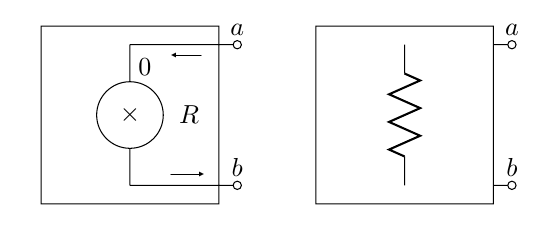
\includegraphics[scale=0.5]{images/resistor}
		\centering
		\caption*{Fonte: Modificado de \cite{Bogason2017}}
	\end{figure}
	
	É importante ressaltar que, mesmo não tendo nenhuma onda refletida, os resistores ainda afetam o comportamento dos circuitos ao alterar o coeficiente de reflexão de conexões série e paralelo com a resistência de sua porta de entrada conforme será mostrado na Seção \ref{secFundWdfComp}.
	
		%=========================================================================
		\subsubsection{Capacitores}
		%=========================================================================
	
	Capacitores são definidos no domínio K em frequência conforme indicado na Equação
	
	\begin{equation}
		\label{eqFundWdfCompCap1}
		Z_c = \frac{1}{s.C} = \frac{V}{I}
	\end{equation}
	
	Novamente utilizando-se das relações indicadas nas Equações \ref{eqFundWdfVar4} e \ref{eqFundWdfVar5} obtêm-se as relações para o domínio W conforme indicado nas Equações \ref{eqFundWdfCompCap2} e \ref{eqFundWdfCompCap3}.
	
	\begin{equation}
		\label{eqFundWdfCompCap2}
		\frac{1}{s.C} = \frac{\frac{A+B}{2}}{\frac{A1-B}{2.R_p}}
	\end{equation}
	
	\begin{equation}
		\label{eqFundWdfCompCap3}
		B = \frac{1-s.C.R_p}{1+s.C.R_p}.A
	\end{equation}
	
	Utilizando a transformação bilinear dada na Equação \ref{eqTransformacaoBilinear} para digitalizar a Equação \ref{eqFundWdfCompCap3} tem-se as Equações \ref{eqFundWdfCompCap4} e \ref{eqFundWdfCompCap5}
	
	
	\begin{equation}
		\label{eqFundWdfCompCap4}
		B = \frac{1-2.f_s\frac{z-1}{z+1}.C.R_p}{1+2.f_s.\frac{z-1}{z+1}.C.R_p}.A
	\end{equation} 
	
	\begin{equation}
		\label{eqFundWdfCompCap5}
		B = \frac{(1-2.f_s.C.R_p)+(1+2.f_s.C.R_p).z^{-1}}{(1+2.f_s.C.R_p)+(1-2.f_s.C.R_p).z^{-1}}.A
	\end{equation}
	
	E finalmente, essa relação entre as ondas \textit{A} e \textit{B} pode ser descrita no domínio tempo conforme a Equação \ref{eqFundWdfCompCap6}
	
	\begin{equation}
		\label{eqFundWdfCompCap6}
		b[n] = \frac{((1-2.f_s.C.R_p).a[n]+(1+2.f_s.C.R_p).a[n-1]-(1-2.f_s.C.R_p).b[n-1])}{1+2.f_s.C.R_p}	\end{equation}
	
	Percebe-se pela Equação \ref{eqFundWdfCompCap6} que a onda refletida em um capacitor é relacionada instantaneamente à onda incidente por um fator $\frac{1-2.f_s.C.R_p}{1+2.f_s.C.R_p}$. Afim de anular essa reflexão instantânea se define a resistência $R_p$ como sendo $\frac{1}{2.f_s.C}$. Assim um capacitor pode ser definido no domínio W conforme indicado nas Equações \ref{eqFundWdfCompCap7} e \ref{eqFundWdfCompCap8} e na Figura \ref{figFundWdfCompCap1} e mostrado o funcionamento interno e o símbolo utilizado para capacitores no domínio W.
	
	\begin{equation}
	\label{eqFundWdfCompCap7}
		B = z^{-1}.A
	\end{equation}
	\begin{equation}
	\label{eqFundWdfCompCap8}
		R_p = \frac{1}{2.f_s.C}
	\end{equation}
	
	\begin{figure}[h]
		\label{figFundWdfCompCap1}
		\caption{Funcionamento interno e símbolo de um capacitor no domínio W}
		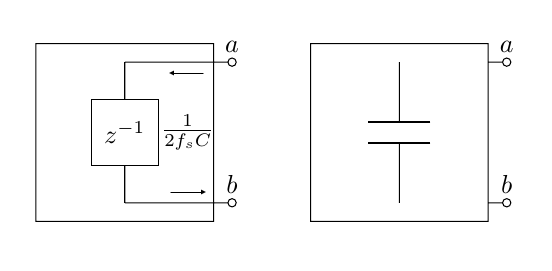
\includegraphics[scale=0.5]{images/capacitor}
		\centering
		\caption*{Fonte: Modificado de \cite{Bogason2017}}
	\end{figure}
	
		%=========================================================================
		\subsubsection{Fonte de tensão com resistência não nula}
		%=========================================================================
	\cite{Yeh2008} Fontes de tensão isolada tem, invariavelmente, uma relação instantânea entre onda incidente e onda refletida, para evitar esse efeito indesejado, é comum na literatura agrupar fontes de tensão com resistores em série conforme o circuito da Figura \ref{figFundWdfCompFontTens1}. Esse circuito pode ser modelado no domínio K conforme o indicado na Equação \ref{eqFundWdfCompFontTens1}.
	
	\begin{equation}
		\label{eqFundWdfCompFontTens1}
		V = V_s + R_s.I
	\end{equation}
	
	 \begin{figure}[h]
		\label{figFundWdfCompFontTens1}
		\caption{Fonte de tensão com resistor em série a ser modelada}
		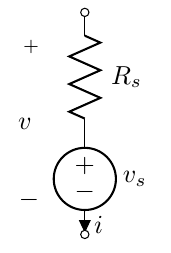
\includegraphics[scale=0.5]{images/fonteTensaoModelada}
		\centering
		\caption*{Fonte: Modificado de \cite{Bogason2017}}
	\end{figure}
	
	Utilizando-se das transformações lineares indicadas nas Equações \ref{eqFundWdfVar4} e \ref{eqFundWdfVar5} e resolvendo as equações de maneira similar à feita anteriormente para resistores e capacitores tem-se que a onde refletida para esse circuito é dada pela Equação 
	
	\begin{equation}
		\label{eqFundWdfCompFontTens2}
		B = 2.\frac{R_p.V_s}{R_p+R_s}-A.\frac{R_p-R_s}{R_p+R_s}
	\end{equation}
	
	Pode-se então definir $R_p = R_s$ de maneira a simplificar a equação e evitar a relação instantânea entre onde incidente e onda refletida. Então, uma fonte de tensão em série com um resistor pode ser descrita no domínio W conforme as Equações \ref{eqFundWdfCompFontTens3} e \ref{eqFundWdfCompFontTens4} e a Figura \ref{figFundWdfCompFontTens2} mostra seu funcionamento e o símbolo utilizado para esse componente.
	\begin{equation}
		\label{eqFundWdfCompFontTens3}
		B = V_s
	\end{equation}
	\begin{equation}
		\label{eqFundWdfCompFontTens4}
		R_p = R_s
	\end{equation}
	
	\begin{figure}[h]
		\label{figFundWdfCompFontTens2}
		\caption{Funcionamento interno e símbolo de uma fonte de tensão com resistência série no domínio W}
		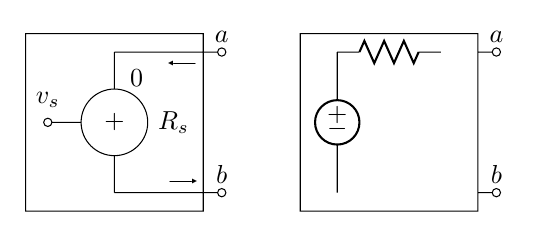
\includegraphics[scale=0.5]{images/fonteTensaoDominioW}
		\centering
		\caption*{Fonte: Modificado de \cite{Bogason2017}}
	\end{figure}
	
		%=========================================================================
		\subsubsection{Fonte de corrente com resistência não nula}
		%=========================================================================
	
	Assim como acontece para fontes de tensão, fontes de correntes independentes tem uma relação instantânea entre onda incidente e onda refletida. Por isso é interessante o uso de fontes de corrente em paralelo com resistores, conforme o circuito da Figura \ref{figFundWdfCompFontCorr1}. As relações entre as grandezas no domínio K para esse circuito são dadas na Equação \ref{TBD}:
	
	\begin{equation}
		\label{eqFundWdfCompFontCorr1}
		V = (I + I_s).R_s
	\end{equation}
	
	\begin{figure}[h]
		\label{figFundWdfCompFontCorr1}
		\caption{Fonte de tensão com resistor em série a ser modelada}
		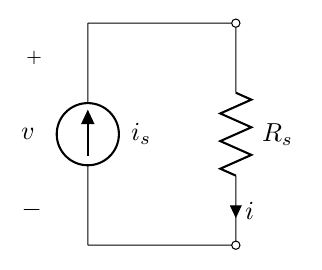
\includegraphics[scale=0.5]{images/fonteCorrenteModelada}
		\centering
		\caption*{Fonte: Modificado de \cite{Bogason2017}}
	\end{figure}
	
	Novamente se utilizando das relações nas Equações \ref{eqFundWdfVar4} e \ref{eqFundWdfVar5} tem-se a relação entre onda incidente e onda refletida indicada na Equação \ref{eqFundWdfCompFontCorr2} :
	
	\begin{equation}
		\label{eqFundWdfCompFontCorr2}
		B = 2.I_s.\frac{R_p.R_s}{R_p+R_s}-a.\frac{R_p-R_s}{R_p+R_s}
	\end{equation}
	
	Novamente, para evitar uma relação instantânea entre onda incidente e onda refletida se define $R_p = R_s$ de maneira que essa fonte de corrente pode ser descrita no domínio W conforme as Equações \ref{eqFundWdfCompFontCorr3} e \ref{eqFundWdfCompFontCorr4} e na Figura \ref{figFundWdfCompFontCorr2} é mostrado seu funcionamento e o símbolo que será usado para este componente no domínio W.
	
	\begin{equation}
		\label{eqFundWdfCompFontCorr3}
		B = I_s.R_s
	\end{equation}
	
	\begin{equation}
		\label{eqFundWdfCompFontCorr4}
		R_p = R_s
	\end{equation}
	
	\begin{figure}[h]
		\label{figFundWdfCompFontCorr2}
		\caption{Funcionamento interno e símbolo de uma fonte de corrente com resistência em paralelo no domínio W}
		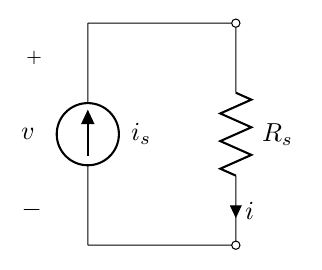
\includegraphics[scale=0.5]{images/fonteCorrenteModelada}
		\centering
		\caption*{Fonte: Modificado de \cite{Bogason2017}}
	\end{figure}
	
	
		%=========================================================================
		\subsubsection{Resumo dos componentes de uma porta}
		%=========================================================================
	A Tabela \ref{tbd} apresente em resumo as características no domínio W para os componentes de 2 portas que serão utilizados neste trabalho.
	
	\todo{adicionar tabela com resumo das características no domínio W para 2 portas}
	
	%=========================================================================
	\subsection{Conexões no domínio W}
	%=========================================================================
	\label{secFundWdfComp}
	
	Nesta seção serão demonstradas as conversões de conexões em série e paralelo do domínio K para o domínio W para conectores de $n$ portas. Novamente como referência são indicados os trabalhos de \citeonline{Bogason2017}, \citeonline{Yeh2008} e  \citeonline{YehTutorial2008} .
	
		%=========================================================================
		\subsubsection{Conexões em série}
		%=========================================================================
		
	Para uma conexão em série conforme indicado na Figura \ref{TBD} se sabe que as correntes e tensões se comportam conforme o indicado na Equação \ref{eqFundWdfConexSer2}.
	
	\begin{equation}
		\label{eqFundWdfConexSer1}
		I_1 = I_2 = ... = I_n
	\end{equation}
	
	\begin{equation}
		\label{eqFundWdfConexSer2}
		\sum_{i=1}^{n} V_i = 0
	\end{equation}
	
	Utilizando-se a definição da Equação \ref{eqFundWdfVar5} na Equação \ref{eqFundWdfConexSer2} e depois utilizando a igualdade dada na Equação \ref{eqFundWdfConexSer1}, tem-se as Equações \ref{eqFundWdfConexSer3} e \ref{eqFundWdfConexSer4}
	
	\begin{equation}
		\label{eqFundWdfConexSer3}
		\sum_{i=1}^{n} (A_i-R_i.I_i) = 0
	\end{equation}
	
	\begin{equation}
		\label{eqFundWdfConexSer4}
		\sum_{i=1}^{n} A_i - I. \sum_{i=1}^{n} R_i = 0
	\end{equation}
	
	Sabendo que todas as correntes são iguais, pode-se então obter a onda refletida para uma porta $\nu$ qualquer aplicando a Equação \ref{eqFundWdfVar5} na Equação \ref{eqFundWdfConexSer4} tendo como resultado a Equação \ref{eqFundWdfConexSer6}.
	
	\begin{equation}
		\label{eqFundWdfConexSer5}
		I_{\nu} = \frac{A_{\nu} - B_{\nu}}{2.R_{\nu}} = \frac{\sum_{i=1}^{n} A_i}{\sum_{i=1}^{n} R_i}
	\end{equation}
	
	\begin{equation}
		\label{eqFundWdfConexSer6}
		B_{\nu} = A_{\nu} -\frac{\sum_{i=1}^{n} A_i}{\sum_{i=1}^{n} R_i}.2.R_{\nu} 
	\end{equation}
	
	Com o objetivo de facilitar a computação das reflexões é comum definir um parâmetro de reflexão que é calculado para cada porta conforme a Equação \ref{eqFundWadfConexSer7} e então a onda refletida nesta porta é dada pela Equação \ref{eqFundWadfConexSer8}:
	
	\begin{equation}
		\label{eqFundWadfConexSer7}
		\gamma_i = \frac{2.R_i}{\sum_{i=1}^{n} R_i}
	\end{equation}
	
	\begin{equation}
		\label{eqFundWadfConexSer8}
		B_{\nu} = A_{\nu} -\gamma_{\nu}.(\sum_{i=1}^{n} A_i)
	\end{equation}
	
	
	Segundo a Equação \ref{eqFundWadfConexSer8} há uma relação instantânea entre onda incidente $A_{\nu}$ e onda refletida $B_{\nu}$ o que como já foi dito é indesejável. 
	
	Quando se faz a conexão de dois conectores série há a criação de loops sem delay, o que torna o filtro digital não realizável. Para evitar esse problema é possível definir uma porta no conector que não terá uma relação instantânea entre onda incidente e refletida, essa porta é denominada Reflection Free Port (RFP).
	
	Para que uma porta seja RFP é necessário forçar sua resistência a ser igual à soma das resistências das demais portas, isso é exemplificado nas Equações \ref{eqFundWadfConexSer9}, \ref{eqFundWadfConexSer10} e \ref{eqFundWadfConexSer11} onde a n-ésima porta é definida como RFP.
	
	\begin{equation}
		\label{eqFundWadfConexSer12}
		R_n = \sum_{i=1}^{n-1} R_i
	\end{equation}  
	
	\begin{equation}
		\label{eqFundWadfConexSer9}
		B_n = A_n -\frac{\sum_{i=1}^{n} A_i}{\sum_{i=1}^{n-1} R_i+R_n}.2.R_n 
	\end{equation}  
	
	\begin{equation}
		\label{eqFundWadfConexSer10}
		B_n = A_n -\frac{\sum_{i=1}^{n} A_i}{2.R_n}.2.R_n 
	\end{equation}
	
	\begin{equation}
		\label{eqFundWadfConexSer11}
		B_n = -(\sum_{i=1}^{n-1} A_i)
	\end{equation}
	
	Também é necessário calcular que a reflexão para as demais portas, que não são RFP, baseando-se no resultado da Equação \ref{eqFundWdfConexSer6}, esse resultado é dado na Equação \ref{eqFundWdfConexSer12} onde esse resultado é calculado para uma porta $\nu$ qualquer.
		
	\begin{equation}
		B_{\nu} = A_{\nu} - 2.\frac{R_{\nu}}{\sum_{i=1}^{n-1} R_i+R_n}.\sum_{i=1}^{n} A_i
	\end{equation}
	
	\begin{equation}
		\label{eqFundWdfConexSer12}
		B_{\nu} = A_{\nu} - \frac{R_{\nu}}{R_n}.\sum_{i=1}^{n} A_i
	\end{equation}
	
	Pode-se então definir um novo $\gamma$ conforme a Equação \ref{eqFundWdfConexSer13} e tem-se a  reflexão simplificadamente de acordo com a Equação \ref{eqFundWdfConexSer14}.
	
	\begin{equation}
		\label{eqFundWdfConexSer13}
		\gamma_{\nu} = \frac{R_{\nu}}{R_n}
	\end{equation} 
	
	\begin{equation}
		\label{eqFundWdfConexSer14}
		B_{\nu} = A_{\nu} - \gamma_{\nu}.\sum_{i=1}^{n} A_i
	\end{equation}

	
		%=========================================================================
		\subsubsection{Conexões em paralelo}
		%=========================================================================
	
	Para uma conexão em paralelo de $n$ elementos conforme indicado na Figura \ref{}, as correntes e tensões podem ser calculadas conforme as Equações \ref{eqFundWdfConexPar1} e \ref{eqFundWdfConexPar2}:
	
	\begin{equation}
		\label{eqFundWdfConexPar1}
		V_1 = V_2 = ... = V_n
	\end{equation}
	
	\begin{equation}
		\label{eqFundWdfConexPar2}
		\sum_{i=1}^{n} I_i = 0
	\end{equation}
	
	Usando a Equação \ref{eqFundWdfVar2} resolvida para $I$, a Equação \ref{eqFundWdfConexPar1} na Equação \ref{eqFundWdfConexPar2} e considerando a admitância $G_i = \frac{1}{R_i}$  tem-se a Equação e \ref{eqFundWdfConexPar4} 
	
	\begin{equation}
		\label{eqFundWdfConexPar3}
		\sum_{i=1}^{n} \big(G_i.(A_i-V_i)\big) = 0;
	\end{equation}
	
	\begin{equation}
		\label{eqFundWdfConexPar4}
		V = \frac{\sum_{i=1}^{n} \big(G_i.A_i\big)}{\sum_{i=1}^{n} \big(G_i\big)}
	\end{equation}
	
	Substituindo então a Equação \ref{eqFundWdfVar4} na Equação \ref{eqFundWdfConexPar4} tem-se finalmente a Equação \ref{eqFundWdfConexPar5} que define a relação entre onda incidente e refletida no conector série para uma porta $\nu$.
	
	\begin{equation}
		\frac{A_{\nu}+B_{\nu}}{2} = \frac{\sum_{i=1}^{n} \big(G_i.A_i\big)}{\sum_{i=1}^{n} \big(G_i\big)}
	\end{equation} 
		
	\begin{equation}
		B_{\nu} = 2.\frac{\sum_{i=1}^{n} \big(G_i.A_i\big)}{\sum_{i=1}^{n} \big(G_i\big)} - A_{\nu}
	\end{equation}
	
	\begin{equation}
		\label{eqFundWdfConexPar6}
		\gamma_i = \frac{2.G_i}{\sum_{j=1}^{n} \big(G_j\big)}
	\end{equation}
	
	\begin{equation}
		A_0 = \sum_{i=1}^{n} \big(\gamma_i.A_i\big)
	\end{equation}
	
	\begin{equation}
		\label{eqFundWdfConexPar5}
		B_{\nu} = A_{\nu} - A_0
	\end{equation}
	
	
	É importante chamar à atenção o fato de que a soma de todos os $\gamma$ calculados de acordo com a Equação \ref{eqFundWdfConexPar6} deve ser igual a 2. Também se percebe pela Equação \ref{eqFundWdfConexPar5} que há uma relação instantânea entre onda incidente $A{\nu}$ e onda refletida $B_{\nu}$, para evitar esse efeito pode-se definir uma porta como RFP forçando sua admitância de entrada a ser igual à soma das admitâncias da demais portas. 
	
	Considerando então que n-ésima porta é RFP e baseando-se na Equação \ref{eqFundWdfConexPar4}, tem-se então a Equação \ref{eqFundWadfConexPar6} que apresenta a onda refletida desta porta e a Equação \ref{eqFundWdtConexPar7} que apresenta a onda refletida para as demais portas. 
	
	\begin{equation}
		  G_{n} = \sum_{i=1}^{n-1} \big(G_i\big)
	\end{equation}
	
	\begin{equation}
		V = \frac{\sum_{i=1}^{n-1} \big(G_i.A_i\big) + \sum_{i=1}^{n-1}\big(G_i.A_i\big).A_n}{2.\sum_{i=1}^{n-1} \big(G_i\big)}	
	\end{equation}
	
	\begin{equation}
		\frac{A_n+B_n}{2} = \frac{\sum_{i=1}^{n-1} \big(G_i.A_i\big) + \sum_{i=1}^{n-1}\big(G_i.A_i\big).A_n}{2.\sum_{i=1}^{n-1} \big(G_i\big)}
	\end{equation}
	
	\begin{equation}
		B_n = \frac{\sum_{i=1}^{n-1} \big(G_i.A_i\big)}{G_n}+A_n.\frac{G_n}{G_n} - A_{n}
	\end{equation}
		
	\begin{equation}
		\gamma_i = \frac{G_i}{G_n}
	\end{equation}
	
	\begin{equation}
		\label{eqFundWadfConexPar6}
		B_n = \sum_{i=1}^{n-1} \big(\gamma_i.A_i\big)
	\end{equation}
	
	\begin{equation}
		B_{\nu} = \frac{\sum_{i=1}^{n-1} \big(G_i.A_i\big)}{G_n}+A_n.\frac{G_n}{G_n} - A_{\nu}	
	\end{equation}
	
	\begin{equation}
		\label{eqFundWdtConexPar7}
		B_{\nu} = B_n + A_n - A_{\nu}
	\end{equation}
	
	
		%=========================================================================
		\subsubsection{Resumo das conexões}
		%=========================================================================
	A Tabela \ref{tbd} apresente em resumo as características no domínio W para os componentes de 2 portas que serão utilizados neste trabalho.
	
	\todo{adicionar tabela com resumo das características no domínio W para 2 portas}
	

	

	%=========================================================================
	\subsection{Não linearidades no domínio W}
	%=========================================================================
	
	%=========================================================================
	\subsection{Amplificadores operacionais no domínio W}
	%=========================================================================
	
	Nesta seção será descrito como simular amplificadores operacionais ideais no domínio W com base no trabalho de \citeonline{Paiva2012}. Há métodos de simulação de amplificadores operacionais capazes de lidar com não idealidades \cite{Werner2015} \cite{Werner2016}, mas estes fogem do escopo deste trabalho. 
	
	
	Amplificadores operacionais (amp op) são componentes amplamente utilizados em eletrônica analógica e especificamente na criação de efeitos de distorção, em conjunto com diodos, que é o foco deste trabalho. Afim de criar um equivalente a este componente para simulação um modelo tradicional é dado na Figura \todo{Adicionar figura do modelo do amplificador} \cite{Boylestad2002}. Neste modelo a fonte de tensão variável depende das tensões nos terminais de entrada positivo e negativo, isso faz com que a solução deste modelo dependa de equações implícitas o que é computacionalmente complexo e, consequentemente, indesejado em processamento de áudio em tempo real.
	
	Analisando as características de um amp op ideal (impedância de entrada infinita, impedância de saída nula e ganho infinito) pode-se assumir que a resistência $R_i$ é infinita (um circuito aberto) e a resistência $R_o$ é nula (um curto circuito). Levando em consideração essas idealidades o modelo do amp op pode ser descrito conforme o conjunto de circuitos da Figura \todo{Adicionar figura modelo do amplificador ideal}. A grande vantagem deste novo modelo é que não existem equações implícitas.
	
	Com base n
	
	
	
	\section{Espaço de Estados}

%=========================================================================
% METODOLOGIA EXPERIMENTAL
	\chapter{Metodologia Experimental}
	
	\section{Pedais a serem modelados}
	
	\section{Modelamento em filtro digital de onda}
	
	\section{Código spice do circuito}
%=========================================================================

%=========================================================================
% RESULTADOS E DISCUSSÕES
	\chapter{Resultados}
	
	\section{Resultados circuito 1}
	
	\section{Resultados circuito 2}
	
%=========================================================================

%=========================================================================
% CONCLUSÃO
	\chapter{Conclusões}
%=========================================================================

%=========================================================================
% PROPOSTA DE TRABALHOS FUTUROS
	\chapter{Propostas de Trabalhos Futuros}
%=========================================================================

%=========================================================================
% REFERÊNCIAS BIBLIOGRÁFICAS
	\
	\bibliography{references}
%=========================================================================

%=========================================================================
% APÊNDICES
	\begin{apendicesenv}
	\partapendices
%=========================================================================
\end{apendicesenv}

%=========================================================================
% ANEXOS
	\begin{anexosenv}
	\partanexos
%=========================================================================
\end{anexosenv}

\end{document}
